\question{Приложения определенного интеграла: вычисление длины дуги кривой (вывод формулы).}

Пусть дана гладкая (без самопересечений, разрывов и циклов) дуга \(\breve{AB}\)
задаваемая уравнением \(y = y(x)\), где \(y(x)\) функция, дифференцируемая на
\([a; b]\). Найдем её длину.

Построим интеграл:
\begin{enumerate}
  \item Дробление \(\breve{AB}\) такими \(M_{i}\), что
  \(A M_{0} \dotsc M_{n} B \approx \breve{AB}\).

  \item Стянем точки \(M_{i - 1}\) и \(M_{i}\) хордой и получим координатный
  треугольник.

  \begin{multicols}{2}
    \begin{align*}
      \Delta l_{i}
      \approx \Delta L_{i}
      = \sqrt{(\Delta x_{i})^2 + (\Delta y_{i})^2}
      = \sqrt{1 + \left(\frac{\Delta y_{i}}{\Delta x_{i}}\right)^2} \Delta x_{i}
    \end{align*}
    \columnbreak

    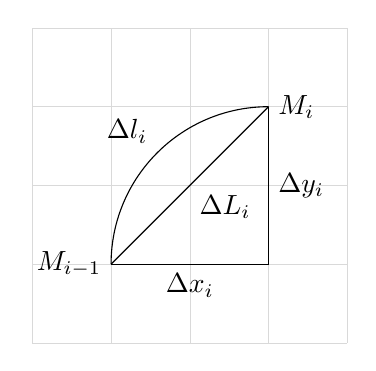
\begin{tikzpicture}  
  \draw[very thin, gray!30, step = 1cm] (0, 0) grid (4, 4);
  \draw (1, 1) -- (3, 1) -- (3, 3);
  \draw (3, 3) arc (90:180:2) node[midway, above left] {\(\Delta l_{i}\)};
  \draw (1, 1) -- (3, 3) node[midway, below right] {\(\Delta L_{i}\)};

  \draw node[below] at (2, 1) {\(\Delta x_{i}\)};
  \draw node[right] at (3, 2) {\(\Delta y_{i}\)};
  \draw node[left] at (1, 1) {\(M_{i - 1}\)};
  \draw node[right] at (3, 3) {\(M_{i}\)};
\end{tikzpicture}

  \end{multicols}

  \item Заметим, что \(\dfrac{\Delta y_{i}}{\Delta x_{i}}\) это отношение
  конечных приращений, поэтому можно применить т. Лагранжа:
  \begin{align*}
    \exists \xi_{i} \in [x_{i - 1}, x_{i}] \colon
      \frac{\Delta y_{i}}{\Delta x_{i}} = f'(\xi_{i})
    \\
    \Delta L_{i}
    = \sqrt{1 + y'(\xi_{i})^2} \Delta x_{i}
  \end{align*}
  
  \item Составим предел интегральных сумм и перейдем к интегралу:

  \begin{align*}
    L = \lim_{\substack{n \to \infty \\ \tau \to 0}}
      \sum_{i = 1}^{n} \sqrt{1 + y'(\xi_{i})^2} \Delta x_{i}
    \implies L = \int_{a}^{b} \sqrt{1 + y'(x)^2} \dd x
  \end{align*}
\end{enumerate}

\begin{remark}\label{arc-diff}
  Выражение \(\dd l = \sqrt{1 + y'(x)^2} \dd x\) называется дифференциалом дуги.
\end{remark}